%!TeX program = lualatex
\documentclass{beamer}
\usetheme{Boadilla}
\usecolortheme{beaver}
\usepackage{amsmath}
\title{Bertrand's Postulate}
\author{Dakota Wicker}
\graphicspath{.}
\usefonttheme{serif}
\newtheorem{lem}{Lemma}
\newtheorem{goal}{Goal}
\newtheorem{defi}{Definition}
\newtheorem{pos}{Bertrand's Postulate}
\usepackage{mathtools}
\DeclarePairedDelimiter\floor{\lfloor}{\rfloor}
\DeclarePairedDelimiter\bigfloor{\bigg\lfloor}{\bigg\rfloor}
\begin{document}

\begin{frame}
\titlepage
\end{frame}

\begin{frame}
\frametitle{History}
\begin{itemize}[<+->]
\item First conjectured by Joseph Bertrand in 1845
\item First proof by Pafnuty Chebyshev in 1850 when exploring P.N.T
\item Shorter but more advanced proof was given by Srinivasa Ramanujan in 1919
\item Central binomial coefficient
\item Short and simple proof given by Paul Erdős in 1932 \\ (20 years old \& first publication)
\end{itemize}
\pause
\begin{center}
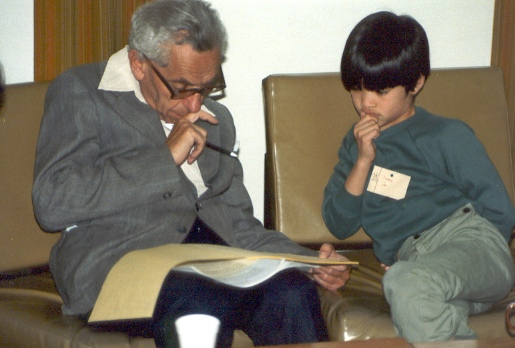
\includegraphics[scale=.5]{Erdos_Tao}
\end{center}
\end{frame}

\begin{frame}

\begin{pos}
\normalfont For any integer $n > 1$, there always exists at least one prime number $p$ such that $ n < p < 2n$.
\end{pos}
\begin{columns}[onlytextwidth,T]
\column{\dimexpr\linewidth-60mm-5mm}\begin{center}
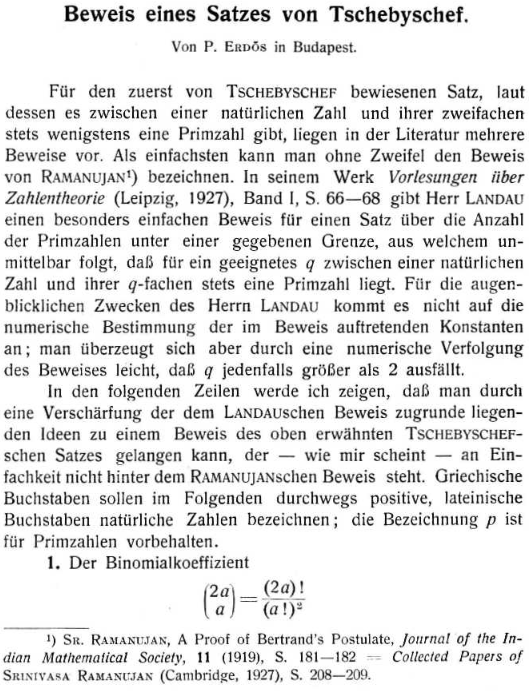
\includegraphics[scale = .30]{proof_german}
\end{center}
\column{\dimexpr\linewidth-60mm-5mm}\begin{center}
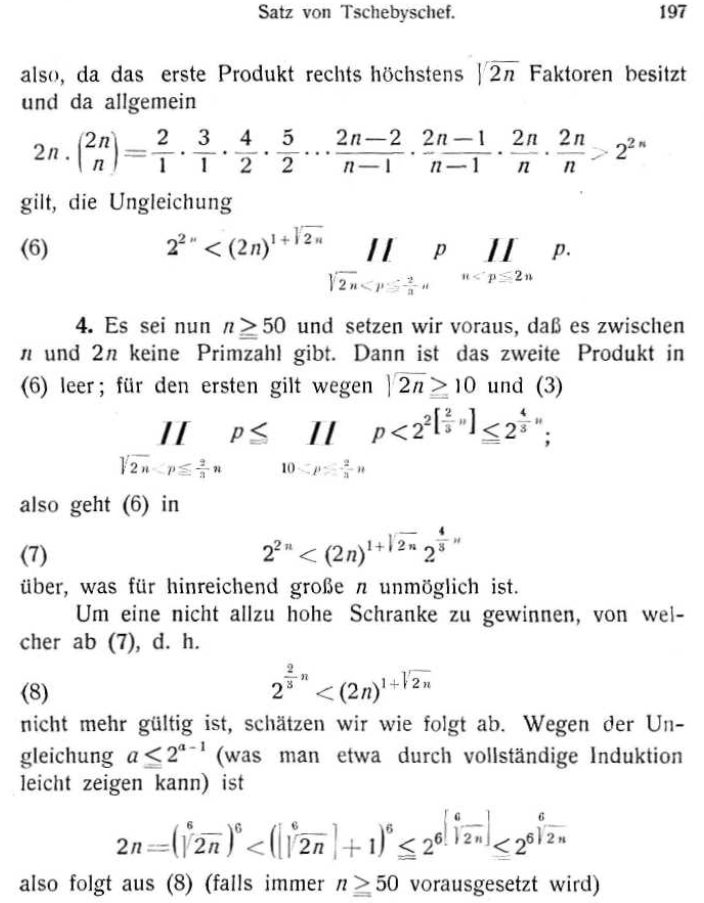
\includegraphics[scale = .22]{proof_german2}
\end{center}
\end{columns}
\end{frame}

\begin{frame}
\begin{lemma}[1]
\normalfont By the binomial theorem,
$${2n \choose n}  \geq \frac{4^n}{2n + 1}$$
 \end{lemma}
\pause
\begin{columns}[onlytextwidth,T]
\column{\dimexpr\linewidth-60mm-5mm} Consider the $(2n+1)$-term sum
 $$\sum_{i=0}^{2n} {2n \choose i}.$$
 \pause
The binomial theorem states that
$$(x + y)^{2n} = \sum_{i=0}^{2n} {2n \choose i} x^{2n - i}y^i$$
Let $x = y = 1$
\column{\dimexpr\linewidth-10mm-0mm} \ \\ \ \\  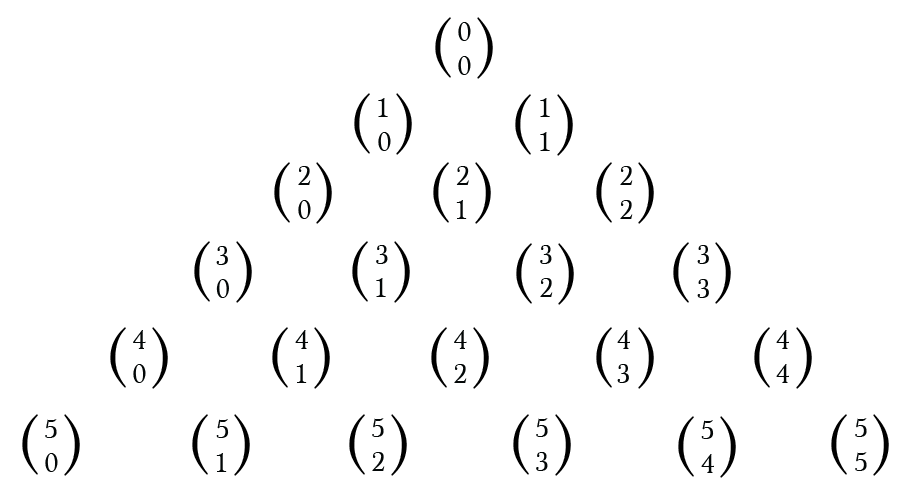
\includegraphics[width=70mm]{pascal2}
\end{columns}
\end{frame}


\begin{frame}
\begin{goal}
\normalfont We know the previous lower bound to be true. We want to show that if there is no prime $p$ with $n < p < 2n$ where $n > 1$, then there is some upper bound on ${2n \choose n}$ that is smaller than $\frac{4^n}{2n+1}$(unless $n$ is small but then computer verifies). This would be a contradiction, so it must be true that there is always prime $p$ with $n < p < 2n.$
\end{goal}
\end{frame}

\begin{frame}
\frametitle{$O_p(n)$}
\begin{defi}
\normalfont Define $O_p(n)$ to be the largest exponent of $p$ that divides $n$.
\end{defi}
\pause
Note: This is the integer exponent on $p$ in the prime factorization of $n$.
\pause
The following properties hold
\pause
\begin{itemize}
\item $O_p(ab) = O_p(a) + O_p(b)$
\pause
\item $O_p\left(\frac{a}{b}\right) = O_p(a) - O_p(b)$
\end{itemize}
\end{frame}

\begin{frame}
\frametitle{Legendre's Formula}
\begin{corollary}[1]
\normalfont Legendre's Formula states that for any prime $p$, and any positive integer $n$, then
$$O_p(n!) = \sum_{i = 1}^{\infty} \bigfloor{\frac{n}{p^i}}.$$
\end{corollary}
\pause
You could think of is saying that since $n!$ is the product of integers 1 through $n$, that $O_p(n!)$ is the amount of multiples of $p$ less than $n$ (which is $\floor{\frac{n}{p}}$). But you actually need to double count for $p^2$ and triple count for $p^3$ and so on.
\end{frame}

\begin{frame}
\frametitle{Example}
Let $n =4$. Then $n! = 4! = 24 = 2^3 \cdot 3^1.$ It follows that
$$O_2(24) = \sum_{i = 1}^{\infty} \bigfloor{\frac{4}{2^i}} = \bigfloor{\frac{4}{2}} + \bigfloor{\frac{4}{2^2}} + \cdots = 2 + 1 + 0 + \cdots = 3.$$
and
\pause
$$O_3(24) = \sum_{i=1}^{\infty} \bigfloor{\frac{4}{3^i}} =\bigfloor{\frac{4}{3}} + \cdots = 1 + 0 + \cdots = 1.$$
\end{frame}

\begin{frame}
\frametitle{Important Fact(s)}
Let 
$$n \geq 3, \text{ and } \frac{2}{3}n < p \leq n.$$
\pause
This actually guarantees that there is one factor of $p$ in $n!$, and two factors of $p$ in $(2n)!.$ Consider $1 < p \leq n < n +1 < 2p \leq 2n$ and 
$${2n \choose n} = \frac{(2n)!}{(n!)(2n - n)!} = \frac{(2n)!}{(n!)^2}  = \frac{2n(2n-1)(2n-2)\cdots(n+1)}{n(n-1)(n-2)\cdots 1}$$
\pause
%By product and quotient rule, this means that
%$$O_p\left({2n \choose n}\right) = O_p\left(\frac{(2n)!}{(n!)^2}\right) = O_p((2n)!) - 2O_p(n!) = 0.$$
which shows that there is no such $p$ such that $p | {2n \choose  n}$ given the inequality. It also shows that there is no prime factor greater than $2n$.
\end{frame}

\begin{frame}
\frametitle{$p^{O_p({2n \choose n})} \leq 2n$}
\begin{lemma}[1]
\normalfont If $p | {2n\choose n}$ then $p^{O_p({2n \choose n})} \leq 2n.$
\end{lemma}
\pause
\begin{proof}
Let $r(p)$ be such that $p^{r(p)} \leq 2n < p^{r(p)+1}$. It follows that
\pause
\vspace{-.4cm}
\begin{align*}
O_p\left({2n \choose n}\right) &= O_p((2n)!) - 2O_p(n!) = \sum_{i=1}^{r(p)}\bigfloor{\frac{2n}{p^i}} - 2\sum_{i=1}^{r(p)}\bigfloor{\frac{n}{p^i}} \\
&= \sum_{i = 1}^{r(p)}\left(\bigfloor{\frac{2n}{p^i}} - 2\bigfloor{\frac{n}{p^i}}\right) \\
&\leq r(p).
\end{align*}
\pause
The last line is justified because for all real $x$, $0 \leq \floor{2x} - 2\floor{x} \leq 1$ which is either 0 or 1. Therefore $p^{O_p\left({2n \choose n}\right)} \leq p^{r(p)} \leq 2n.$
\end{proof}
\end{frame}

\begin{frame}
\begin{corollary}[2]
\normalfont The number of prime numbers dividing ${2n \choose n}$, $\ell$, is at least $\frac{\log_2{2n\choose n}}{\log_2(2n)}$
\end{corollary}
\pause
\begin{proof}
Let $p_1, ..., p_{\ell}$ be the distinct primes dividing ${2n \choose n}.$ It follows that
\pause
$${2n \choose n} = \prod_{i = 1}^{\ell}p_i^{O_{p_i}({2n\choose n})} \leq (2n)^\ell$$
because of Lemma (1).
\end{proof}
\end{frame}

\begin{frame}
\frametitle{Product of Primes}
\begin{corollary}[3]
\normalfont For all $n \geq 2$, $\displaystyle\prod_{p \leq n} p \leq 4^n$, where the product is over primes.
\end{corollary}
\pause
\begin{proof}\renewcommand{\qedsymbol}{}
We proceed by induction. When $n = 2$, $\displaystyle\prod_{p\leq2} p = 2 \leq 4^2.$ Now assume that it works for $n-1$.
\pause
\ \\
When $n$ is even, it follows that
$$\prod_{p \leq n-1} p = \prod_{p \leq n} p \leq 4^{n-1} \leq 4^n.$$
When $n$ is odd, we work with $n = 2m +1...$
\end{proof}
\end{frame}

\begin{frame}
\frametitle{Product of Primes}
\begin{proof}\renewcommand{\qedsymbol}{}
When $n = 2m + 1$, I know that
\pause
$$\prod_{p \leq n}p = \prod_{p\leq m+1}p  \prod_{m+2 \leq p \leq 2m + 1}p$$
\pause
By the induction hypothesis and $n-1 = 2m$, $\displaystyle\prod_{p\leq m+1}p \leq 4^{m+1}$. \pause Also because\vspace{-.3cm}
$${2m+1 \choose m} = \frac{(2m+1)!}{(m+1)!} = (2m+1)(2m)\cdots (m+2),$$
this shows that that all primes between $m+2$ and $2m + 1$ divide ${2m +1 \choose m}$ it must be true that...

\end{proof}
\end{frame}

\begin{frame}
\frametitle{Product of Primes}
\begin{proof}\renewcommand{\qedsymbol}{}
$$\prod_{p\leq n}p \leq 4^{m+1} {2m+1 \choose m}.$$
\pause
Suppose ${2m+1 \choose m} > 2^{2m}.$ 
\pause
Then since $2m +1$ is odd 
$${2m+1 \choose m} + {2m+1 \choose m +1} = 2{2m+1 \choose m} > 2(2^{2m}) = 2^{2m + 1}$$
But,
\pause
$$\sum_{i = 1}^{2m +  1} {2m+1 \choose i} = 2^{2m + 1}$$
and $n \geq 2$, so $2m + 1 \geq 3$, and so this is a 3-term sum so there is a contradiction. Therefore ${2m+1 \choose m} \leq 2^{2m}.$
\end{proof}
\end{frame}

\begin{frame}
\begin{proof}
\frametitle{Product of Primes}
I have that 
$$\prod_{p\leq n}p \leq 4^{m+1} {2m+1 \choose m}$$
and ${2m+1 \choose m} \leq 2^{2m}.$ Therefore I conclude that
$$\prod_{p\leq n}p \leq 4^{m+1}  2^{2m} = 4^{2m + 1} = 4^n$$
This concludes the proof.
\end{proof}
\end{frame}

\begin{frame}
\center{BREAK!}
\center{What have we learned?}
\pause
\begin{itemize}[<+->]
\item $\frac{4^n}{2n + 1} \leq {2n\choose n}$.
\item If $p|{2n\choose n}$ then $p^{O_p({2n\choose n})} \leq 2n.$
\item If $n \geq 3,$ and $\frac{2}{3}n < p \leq n$ there is no $p$ such that $p | {2n\choose n}$.
\item If $n \geq 3,$ and $\frac{2}{3}n < p \leq n$ there is no prime factor greater than $2n$.
\end{itemize}
\end{frame}

\begin{frame}
\frametitle{The Proof}
\begin{proof}\renewcommand{\qedsymbol}{}
We will now prove Bertrand's Postulate.
Let $n \geq 3$ be such that there is no prime $p$ with $n < p \leq 2n$. Then \pause
$$ {2n \choose n} \leq (2n)^{\sqrt{2n}} \prod_{\sqrt{2n} < p \leq 2n/3}p$$\pause
Note that ${2n \choose n}$ has at most $\sqrt{2n}$ prime factors that do not exceed $\sqrt{2n}.$ By Lemma 1, the most a prime factor can contribute is $2n$. Now, our hypothesis says that there is no $p$ such that $n < p \leq 2n$. Finally, remember now, the important fact!, if $n \geq 3$, and $\frac{2}{3}n < p \leq n$, then there is no prime factors of ${2n \choose n}$ between $\frac{2}{3}n$ and $n$ or greater than $2n$.
\end{proof}
\end{frame}

\begin{frame}
\frametitle{The Proof}\renewcommand{\qedsymbol}{}
\begin{proof}
Conveniently multiplying by more terms, it must also be true that
$${2n \choose n } \leq (2n)^{\sqrt{2n}} \prod_{p\leq \frac{2}{3}n}p $$
\pause
and using Corollary 3, it follows that
$${2n \choose n} \leq (2n)^{\sqrt{2n}} 4^{\frac{2}{3}n}.$$
\end{proof}
\end{frame}

\begin{frame}
\frametitle{The Proof}\renewcommand{\qedsymbol}{}
\begin{proof}
\begin{center} BUT WAIT  \end{center}\pause
From one of the very first slides it is shown to be true that 
$$\frac{4^n}{2n + 1} \leq {2n \choose n} $$
\pause
and I have just shown that if there is no $p$ such that $n < p \leq 2n$
$${2n \choose n} \leq (2n)^{\sqrt{2n}}4^{\frac{2}{3}n} $$
\pause
So,
$$\frac{4^n}{2n+1} \leq (2n)^{\sqrt{2n}}4^{\frac{2}{3}n}.$$
\end{proof}
\end{frame}

\begin{frame}
\begin{proof}
$$\frac{4^n}{2n+1} \leq (2n)^{\sqrt{2n}}4^{\frac{2}{3}n} $$
BUT this inequality fails! Specifically for all $n \geq 468$. Therefore there is a contradiction, and so it is concluded that  there exists a $p$ such that $n < p < 2n$ given $n \geq 468.$ For all $n < 468$ this is verified by manually checking  the following primes satisfy the theorem for all $n < 468.$
$$2,3,5,7,13,23,43,83,163,317,631.$$
\end{proof}
\end{frame}

\begin{frame}
\frametitle{Applications}
\begin{theorem}[1.1]\normalfont 
The set of integers $\{1,2,3,\cdots,2n\}, n \geq 1$ can be partitioned into pairs $\{a_i, b_i \}$ such that $a_i + b_i$ is prime for all $i = 1,2,\cdots,n$.
\end{theorem}
\pause
\begin{theorem}[1.2]\normalfont 
There are infinitely many $G_{2n}$'s that have a Hamiltonian cycle. (Not neccesarily all $G_{2n}$)
\end{theorem}
\begin{center}
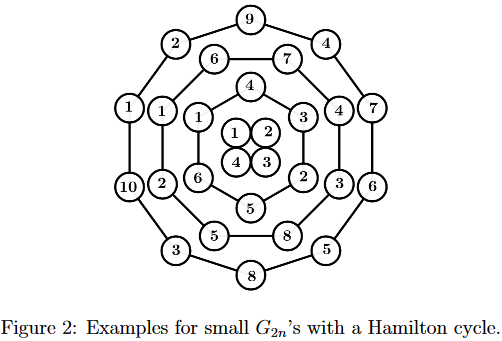
\includegraphics[scale=.4]{g2n}
\end{center}
\end{frame}

\begin{frame}
\frametitle{Applications}
\begin{theorem}[1.3]\normalfont
$G_{2n}, \ n \geq 2$ contains a Hamiltonian cycle if there exists two primes $p_1 < p_2 $ in $[1,2n]$ such that $2n + p_1$ and $2n + p_2$ are primes and $\gcd{(\frac{p_2 - p_1}{2},n)} = 1.$
\end{theorem}
\pause
\begin{theorem}[2]\normalfont
$n$'th Harmonic Number is not an integer, $ n \geq 2$.
\end{theorem}
\end{frame}

\begin{frame}
\begin{center}
Questions?
\end{center}
\end{frame}
\end{document}